\chapter{Conceptos previos}
\label{conceptos}

En este capítulo se abordan conceptos necesarios para poder comprender las soluciones a los problemas comunes que se trataran luego. Entre ellos se encuentran algunas definiciones como la de \textit{Sistemas embebidos} y otras relacionadas a la IS. También, conceptos centrales del diseño para el cambio y todo lo necesario para llevarlo a cabo.


\section{Sistemas embebidos}
Distintos autores proponen diferentes definiciones de sistemas embebidos:
\\\\
\noindent
``\textit{Un sistema computarizado dedicado a realizar un conjunto específico de funciones del mundo real, en lugar de proporcionar un entorno de computación generalizado.}''~\cite{douglass}
\\\\
\noindent
``\textit{Un sistema embebido es un sistema computarizado diseñado específicamente para su aplicación.}'' Debido a que su misión es más limitada que la de una computadora de propósito general, un sistema embebido tiene menos soporte para aspectos no relacionados con la ejecución de la aplicación.~\cite{elecia}
\\\\
\noindent
``\textit{Un sistema embebido es un sistema informático aplicado, a diferencia de otros tipos de sistemas informáticos como las computadoras personales (PCs) o las supercomputadoras.}''~\cite{noergaard2005embedded}
\\\\
\noindent		
El último autor comenta que los sistemas embebidos cumplen las siguientes afirmaciones:
\begin{itemize}
	\item Los sistemas embebidos son más limitados en funcionalidad de hardware y/o software que una computadora personal.
	\item Un sistema embebido está diseñado para realizar una función dedicada.
	\item Un sistema embebido es un sistema informático con requisitos de mayor calidad y fiabilidad que otros tipos de sistemas informáticos.
	\item Algunos dispositivos que se denominan sistemas embebidos, como los \gls{pda}.
\end{itemize}

De las definiciones se puede concluir que un sistema embebido es una pieza clave que permite que hardware especializado cumpla con su propósito específico. A diferencia de los sistemas de propósito general, el software en un sistema embebido está diseñado para interactuar estrechamente con los componentes de hardware, respondiendo en tiempo real a eventos del entorno, ya sea para controlar actuadores, monitorear sensores o gestionar comunicaciones. Este software está optimizado para requisitos específicos como velocidad, consumo energético, y confiabilidad, lo que lo hace esencial en aplicaciones críticas como dispositivos médicos, sistemas automotrices y controles industriales.
	
En resumen, el software de un sistema embebido actúa como el cerebro que dirige y coordina los recursos del hardware para realizar funciones concretas. En la tabla~\ref{tab:ejSistEmbebidos} encontramos ejemplos de dispositivos en los que se utilizan sistemas embebidos extraída de \cite{noergaard2005embedded}.

\begin{table}[h]
\caption{Ejemplos sistemas embebidos.}
    \centering
    \label{tab:ejSistEmbebidos}
    \begin{tabular}{|l|l|}
        \hline
        \textbf{Mercado} & \textbf{Dispositivo Embebido} \\ \hline
        Automotriz & Sistema de encendido \\ 
        & Control del motor \\ 
        & Sistema de frenos (Sistema Antibloqueo de Frenos - ABS) \\ \hline
        Electrónica de consumo & Decodificadores (DVDs, VCRs, Cajas de cable, etc.) \\ 
        & Asistentes Personales Digitales (\gls{pda}) \\ 
        & Electrodomésticos (Refrigeradores, Tostadoras, Microondas) \\ 
        & Automóviles \\ 
        & Juguetes/Juegos \\ 
        & Teléfonos/Celulares/Bípers \\ 
        & Cámaras \\ 
        & Sistemas de Posicionamiento Global (GPS) \\ \hline
        Control Industrial & Sistemas de control y robótica (Manufactura) \\ \hline
        Médico & Bombas de infusión \\ 
        & Máquinas de diálisis \\ 
        & Prótesis \\ 
        & Monitores cardíacos \\ \hline
        Redes & Routers \\ 
        & Hubs \\ 
        & Puertas de enlace \\ \hline
        Automatización de Oficina & Máquinas de fax \\ 
        & Fotocopiadoras \\ 
        & Impresoras \\ 
        & Monitores \\ 
        & Escáneres \\ \hline
    \end{tabular}
\end{table}

Otros autores \cite{lee2017introduction} describen sistemas \textit{ciber-físicos} (\Ac{CSP}\footnote{por sus siglas en inglés (cyber-physical system)}) como la integración de la computación con procesos físicos. Esta integración usualmente se lleva a cabo utilizando sistemas embebidos con ciclos de retroalimentación; en los cuales la parte computacional afecta al ámbito físico y viceversa. Los componentes que permiten la comunicación entre ambos mundos son sensores y actuadores.
Además, si tomamos en cuenta los ejemplos que se presentan tanto en \cite{noergaard2005embedded} como en \cite{lee2017introduction}, podemos decir que la mayoría de los sistemas embebidos realizan tareas de \textbf{control} sobre el mundo físico.

Con respecto al hardware en donde corren los sistemas embebidos podemos descatar que suele consistir en una placa o chip compacto que incluye:
\begin{itemize}
    \item \textbf{Unidad de Microcontrolador (MCU):} Un microcontrolador que integra un procesador, memoria y perif\'ericos en un solo chip. Es el componente principal que ejecuta el software.
    \item \textbf{Memoria Flash:} Utilizada para almacenar el programa y los datos no vol\'atiles.
    \item \textbf{Memoria RAM:} Proporciona almacenamiento temporal para datos en tiempo de ejecuci\'on.
    \item \textbf{Interfaces de entrada/salida:} Puertos \gls{GPIO}, \gls{ADC}, \gls{PWM} y otros para interactuar con sensores, actuadores y otros dispositivos externos.
    \item \textbf{Fuente de Energ\'ia:} Puede provenir de bater\'ias, adaptadores de corriente o incluso energ\'ia recolectada del entorno.
\end{itemize}
El tama\~no compacto y la integraci\'on de componentes distinguen a los sistemas embebidos de otros sistemas m\'as grandes como las computadoras de escritorio o los servidores. Se diferencian, además, en su poder de computo limitado tanto por el hardware (baja disponibilidad de memoria RAM, \gls{clock} de la CPU bajo, etc) como por la disponibilidad de energía eléctrica.

Existen varios microcontroladores multipropósito de uso comercial, tales como los producidos por la empresa Arduino \cite{arduinoMicro} o los similares de la familia  Raspberry Pi \cite{raspMicro}. La presentación de los mismos suele ser en forma de una placa preparada para conectar los inputs y outputs, como las que se observan en figuras \ref{arduinoUNO} y \ref{raspberry}.

Por defecto, el microcontrolador ejecuta el software almacenado en su unidad flash, la cual debe ser grabada cada vez que se actualice el código. Dado esto y las limitaciones de hardware ya mencionadas, se deben tener ciertas consideraciones a la hora de escribir el código. Tales como, prestar atención a la performance del sistema, a la cantidad de librerías a utilizar, al uso de memoria RAM, etc.

\begin{figure}[h!]
	\caption{Arduino UNO}
	\label{arduinoUNO}
	\centering
    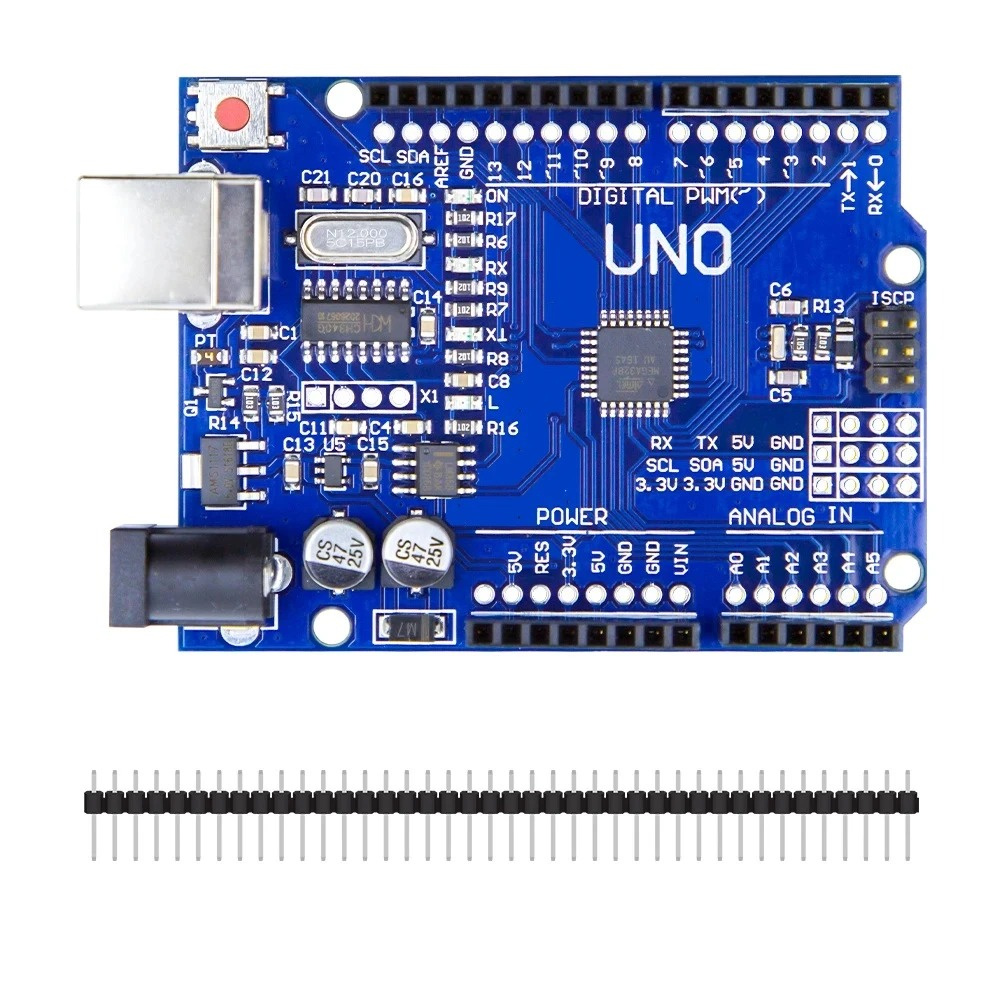
\includegraphics[width=0.5\linewidth]{arduinoUNO.jpeg}
\end{figure}


\begin{figure}[h!]
	\caption{Raspberry Pico 2}
	\label{raspberry}
	\centering
    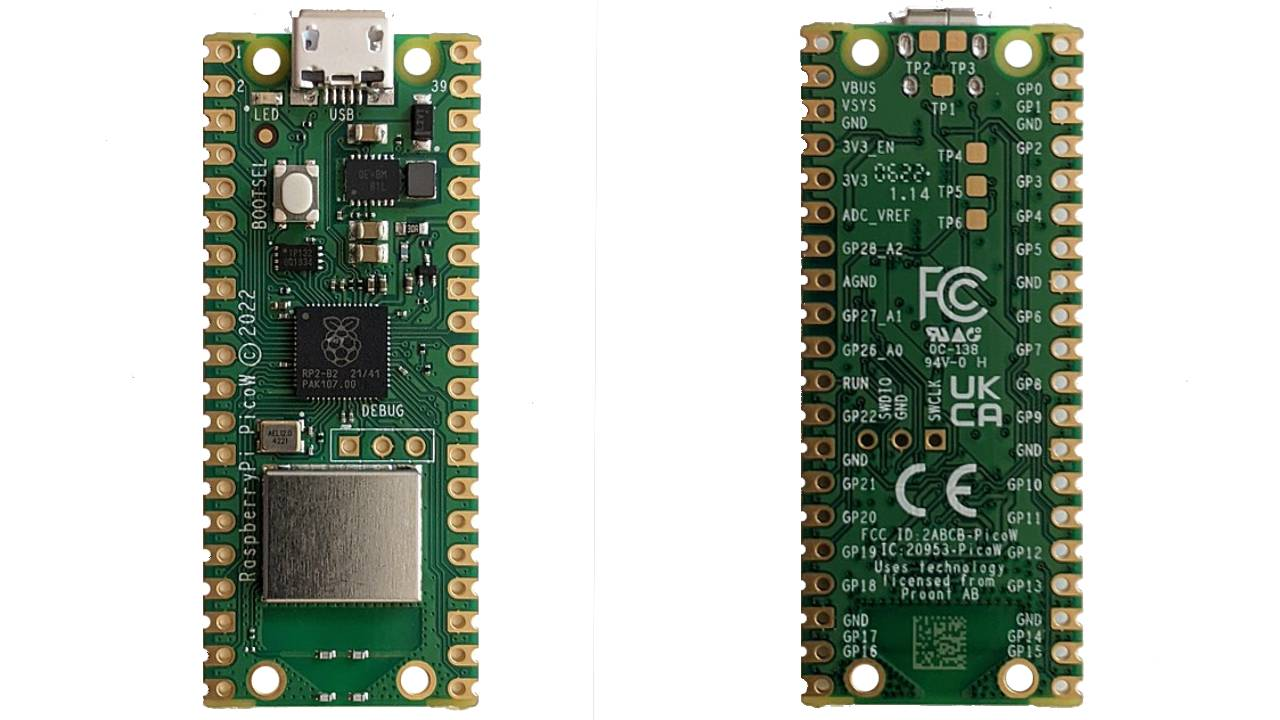
\includegraphics[width=0.6\linewidth]{raspberry_pico2.jpg}
\end{figure}


\subsection{Interrupciones}
Las interrupciones en un microcontrolador son eventos que pausan la ejecución del programa principal para atender una tarea urgente. Funcionan como un mecanismo de respuesta automática que permite que el microcontrolador responda inmediatamente a eventos externos o internos sin depender de que el programa principal revise continuamente el estado de los dispositivos o variables asociadas a la generación de la interrupción.

Cuando ocurre una interrupción (por ejemplo, un cambio en un sensor o una solicitud de un actuador), el microcontrolador detiene su ejecución actual y salta a una rutina de interrupción (ISR, Interrupt Service Routine), ver diagrama de la figura \ref{interrupt}. Esta rutina es un fragmento de código predefinido que realiza las tareas necesarias, como leer un sensor o activar un actuador. Después de ejecutar la ISR, el microcontrolador regresa automáticamente al punto donde fue interrumpido, reanudando el programa principal sin perder el flujo de ejecución.

\begin{figure}[h!]
	\centering
    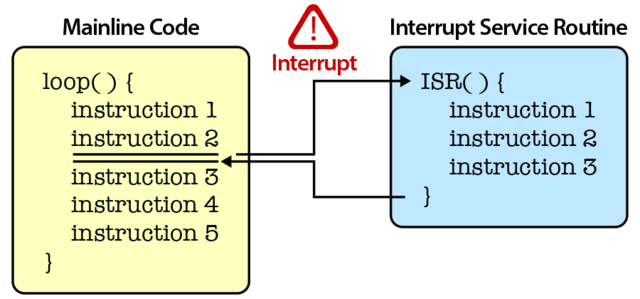
\includegraphics[width=0.7\linewidth]{components_interrupt.png}
    \caption{Diagrama interrupción extraído de \cite{imgInterrupciones}.}
    \label{interrupt}
\end{figure}

Este mecanismo es esencial en sistemas embebidos, especialmente en aquellos que controlan sensores y actuadores, porque permite un control eficiente de múltiples dispositivos. Por ejemplo, un microcontrolador podría usar interrupciones para:

\begin{itemize}
    \item Leer la temperatura de un sensor cada vez que detecta un cambio.
    \item Activar un motor o alarma inmediatamente al detectar un evento específico.
\end{itemize}

Gracias a las interrupciones, el microcontrolador puede realizar tareas en tiempo real y responder rápidamente a eventos críticos, asegurando un control preciso de los sensores y actuadores sin necesidad de monitorear activamente cada dispositivo constantemente.


\section{Ingeniería de Software}
\label{ingso}

La arquitectura y el diseño del software se consideran herramientas esenciales para lograr atributos importantes de calidad del software, como la modificabilidad, reusabilidad, mantenibilidad, etc.\cite{ShawGarlan1996, ghezzi2003, bass2003, DBLP:books/daglib/0030743}
Tradicionalmente, el software para robots tiende a desarrollarse de manera monolítica, con pocas funciones de gran tamaño y numerosas sentencias condicionales anidadas, o mediante una descomposición funcional básica que resulta ineficiente para mantener y reutilizar componentes \cite{code-1,code-2}. Frente a esto, se propone un diseño sistemático basado en principios de la ingeniería de software, aplicados para anticipar y manejar los cambios \cite{Gamma:1995:DPE:186897, DBLP:books/lib/BuschmannHS07}.

El diseño para el cambio, como principio fundamental, se centra en prever modificaciones probables en el software \cite{Parnas1972, ShawGarlan1996, ghezzi2003, bass2003, DBLP:books/daglib/0030743}, por cambios en los objetivos de comportamiento, en el hardware o en los algoritmos de control, entre otros. Diseñar anticipando estos cambios permite reducir los esfuerzos necesarios para implementar ajustes y facilita la reutilización de componentes en familias de software\footnote{en este caso familias de robots} que comparten funcionalidades similares, pero no iguales, y adaptadas a diferentes plataformas de hardware \cite{Parnas02, DBLP:books/daglib/0019719}.

Para abordar estos retos, el diseño modular es clave \cite{Parnas1972}.
Un \textbf{módulo} es un elemento de diseño que, en un lenguaje de programación orientado a objetos, suele implementarse como una \textbf{clase}. A su vez, una \textbf{instancia} de un módulo, en este tipo de lenguajes, corresponde a un \textbf{objeto}. Sin embargo, cuando se habla de diseño, el término adecuado es módulo e instancia, ya que la implementación podría realizarse en un lenguaje que no sea orientado a objetos. Este enfoque de diseño organiza el software como un conjunto de módulos simples con responsabilidades claramente definidas y relaciones explícitas entre ellos. Cada módulo se diseña para ocultar información específica y gestionar un cambio probable de forma aislada, lo que minimiza el impacto de las modificaciones en el resto del sistema. Por ejemplo, si un sensor cambia su forma de reportar datos, el ajuste debería limitarse al módulo responsable de interactuar con ese sensor.

Además, el principio de diseño abierto-cerrado \cite{DBLP:books/ph/Meyer97} se implementa para garantizar que el sistema pueda extenderse mediante nuevos módulos en lugar de modificar los existentes, reduciendo el riesgo de introducir errores al alterar componentes ya probados. Es decir, que un sistema debe estar abierto a extensiones pero cerrado a modificaciones. Esto se complementa con la aplicación de patrones de diseño y estilos arquitectónicos, que aportan soluciones probadas para manejar cambios recurrentes en dominios específicos \cite{Gamma:1995:DPE:186897, DBLP:books/lib/BuschmannHS07}. Por ejemplo, en sistemas robóticos, un estilo arquitectónico basado en bucles de control puede destacar las características esenciales del sistema y facilitar decisiones de diseño óptimas \cite{ShawGarlan1996}.

\subsubsection*{Herencia de Interfaz}
En el diseño modular, un módulo consta de una interfaz y una implementación. La interfaz define el conjunto de métodos accesibles externamente, mientras que la implementación gestiona como el módulo realizar los comportamientos de cada método definido en la interfaz.

Existen esencialmente dos tipos de herencia:

\begin{itemize}
\item \textbf{Herencia de clases}: Un módulo hijo hereda tanto la interfaz como la implementación de un módulo padre, es decir, hereda todo su comportamiento. Si bien esto permite la reutilización de código, introduce un acoplamiento fuerte y reduce la flexibilidad ante cambios, lo que se una mala práctica.
\item \textbf{Herencia de interfaces}: En este caso, un módulo hijo solo hereda la interfaz, permitiendo que cada módulo implemente su propio comportamiento. Este enfoque es más flexible y facilita la adaptabilidad del sistema.
\end{itemize}


\subsubsection*{Composición}
La composición consiste en estructurar sistemas combinando módulos a través de sus interfaces en lugar de depender de relaciones de herencia. Esto se logra mediante la inclusión de referencias a otros dentro de una clase, lo que permite que las instancias deleguen tareas a estos módulos asociados. La composición es una solución que favorece la flexibilidad, ya que evita el acoplamiento jerárquico y permite reemplazar componentes sin afectar el resto del sistema. Además, este enfoque está alineado con el principio de diseño ``preferir la composición sobre la herencia'' \cite{Gamma:1995:DPE:186897}, que enfatiza la modularidad y la apertura al cambio.

Dado que la herencia de clases tiende a ser rígida, los patrones de diseño la evitan, combinando en su lugar herencia de interfaces con composición de módulos y delegación de responsabilidades. Mediante la composición, un módulo puede reutilizar funcionalidad sin necesidad de heredar implementación, mientras que la delegación permite distribuir tareas entre distintos módulos de manera flexible.


\subsection{Metodología de Parnas}
\label{metoParnas}

La metodología de \textbf{Parnas}\cite{Parnas1972}, conocida como Diseño Basado en Ocultación de la Información (\gls{dboi}), es una estrategia de diseño modular que tiene como objetivo preparar los sistemas de software para gestionar el cambio de manera eficiente y con el menor costo posible. Esta metodología parte del principio de que los requerimientos de un sistema no son inmutables, sino que evolucionarán durante su vida útil. Por ello, el diseño debe anticipar y facilitar la incorporación de cambios sin comprometer la integridad del sistema.

\noindent\fbox{\begin{minipage}{\textwidth}
Principio de Ocultación de la Información: Los ítem con alta probabilidad de cambio son el fundamento para descomponer un sistema en módulos. Cada módulo de la descomposición debe ocultar un \textbf{único} ítem con alta probabilidad de cambio, y debe ofrecer a los demás módulos una interfaz insensible a los cambios anticipados. \cite{Parnas1972}
\end{minipage}} 
\\\\
\indent
El núcleo de esta metodología es la identificación de los ítems con alta probabilidad de cambio dentro del sistema. Estos ítems representan aspectos de diseño o implementación susceptibles de modificaciones futuras, como algoritmos, estructuras de datos, interfaces con hardware o incluso requerimientos del usuario (ver lista extendida en sección \ref{listaItems}). Una vez identificados, Parnas sugiere ocultar y aislar cada item de cambio en un módulo independiente, asegurando que cada módulo oculte las decisiones de diseño específicas que podrían cambiar. Esto se logra diseñando interfaces que no expongan detalles de implementación, permitiendo que los módulos interactúen sin conocer sus detalles internos.

La razón por la que queremos aplicar esta metodología es clara: minimizar los costos asociados al desarrollo y mantenimiento del software. Al aislar las áreas susceptibles de cambio, cualquier modificación futura afectará únicamente al módulo correspondiente, sin propagarse al resto del sistema. Además, esta aproximación mejora la capacidad de escalar el sistema, facilita la colaboración en equipos de desarrollo grandes y permite que diferentes programadores trabajen en módulos específicos de manera independiente.

La metodología de Parnas nos ayuda a diseñar para el cambio porque impone una disciplina clara en la forma en que los módulos se estructuran e interactúan. Al encapsular\footnote{Encapsular funcionalidades como el principio de ocultar los detalles internos de un módulo y exponer solo lo necesario a los demás módulos del sistema. La idea clave es que cada módulo tenga una interfaz bien definida y que sus detalles internos (implementación, estructuras de datos, algoritmos) sean ocultos.} las decisiones de diseño que podrían cambiar, evitamos la degradación de la integridad conceptual del sistema y reducimos significativamente el riesgo de introducir errores al realizar modificaciones. En definitiva, el \gls{dboi} fomenta un diseño robusto y adaptable, preparado para enfrentar la evolución inevitable de los sistemas de software.


Los pasos de la metodología son:

\begin{enumerate}
	\item Identificar los ítem con probabilidad de cambio presentes en los requerimientos.
	\item Analizar la diversas formas en que cada ítem puede cambiar.
	\item Se asigna una probabilidad de cambio a cada variación analizada.
	\item Aislar en módulos separados los ítem cuya probabilidad de cambio sea alta; implícitamente este punto indica que en cada módulo se debe aislar un único ítem con probabilidad de cambio.
	\item Diseñar las interfaces de los módulos de manera que resulten insensibles a los cambios anticipados.

\end{enumerate}



\subsection{Items de cambio comunes}
\label{listaItems}

Cuando se diseña pensando en el cambio, una tarea que se agrega es identificar las características o requerimientos del sistema que pueden variar en el tiempo. Naturalmente existen elementos que son mas probables a cambiar que otros, por lo que resulta importante anticiparse a esos cambios en particular. Algunos autores mencionaron algunos items de cambio comunes entre múltiples sistemas \cite{Parnas02}.

\begin{itemize}
	\item Contracción o extension de requisitos.
	\item Configuraciones de hardware.
	\item Formato de los datos de entrada y salida.
	\item Estructuras de datos.
	\item Algoritmos.
	\item Algunos usuarios pueden requerir solo un subconjunto de los servicios o características que otros usuarios necesitan.
	\item Dispositivos periféricos.
	\item Entorno socio-cultural (moneda, impuestos, fechas, idioma, etc.).
	\item Cambios propios del dominio de aplicación.
	\item Cambios propios del negocio de la compañía desarrolladora.
	\item Interconexión con otros sistemas.
\end{itemize}

Es útil consultar estos items a la hora de diseñar siguiendo los criterios de modularización de \cite{Parnas1972}.

\subsection{Documentación}

Quienes diseñan un sistema no serán necesariamente quienes lo implementen, por lo que sus decisiones deben estar disponibles para que diversos interesados en el sistema puedan revisarlas y comprenderlas. Por ello, documentar o describir el diseño de manera adecuada es tan importante como el diseño mismo. En este sentido, Parnas introduce el concepto de ``\textit{design through documentation}'' \cite{parnasDoc}, lo que nos lleva a enunciar el siguiente principio de diseño: \textit{Un diseño sin documentación carece de utilidad práctica.}

Para lograr una buena descripción del diseño se utilizan múltiples documentos que aportan información sobre distintos aspectos a tener en cuenta \cite{ClementsEtAl2010}, entre ellos se encuentran:

\begin{itemize}
\item \textbf{Documentos de módulos}. Los elementos de estos documentos son módulos o unidades de implementación. Los módulos representan una forma basada en el código de considerar al sistema. Cada módulo tiene asignada y es responsable de llevar adelante una función.
\item \textbf{Documentos de aspectos dinámicos}. En estos documentos los elementos son componentes presentes en tiempo de ejecución y los conectores que permiten que los componentes interactúen entre sí.
\item \textbf{Documentos con referencias externas}. Estos documentos muestran la relación entre las partes en que fue descompuesto el sistema y elementos externos (tales como archivos, procesadores, personas, etc.).
\item \textbf{Documentos de módulos}. Especificación de Interfaces, Estructura de Módulos, Guía de Módulos, Estructura de Herencia y Estructura de Uso.
\item \textbf{Documentos de aspectos dinámicos}. Estructura de Procesos, Estructura de Objetos, Diagrama
de Interacciones.
\item \textbf{Documentos con referencias externas}. Estructura Física o de Despliegue
\end{itemize}

A fines didácticos la tesina se centrará, al igual que los patrones, en módulos, interfaces y sus relaciones. Por lo que se utilizarán diagramas de módulos a fin de documentar. Estos consisten en cajas nombradas en las cuales se define la interfaz de un módulo. Ademas, utilizando un conjunto de flechas se determinan sus relaciones.

En los diagramas (o figuras) se utilizan los siguientes símbolos. 

\begin{tabular}{m{0.3\linewidth} p{0.6\linewidth}}
\hline
&\\[-0.2cm]
& \textbf{Significado de los símbolos}\\
\hline
&\\
\begin{tikzpicture}\sf
\umlsimpleclass{A}
\umlsimpleclass[below=0.5cm of A]{B}
\umlVHVinherit{B}{A}
\end{tikzpicture} & {\modFCFont B} hereda de {\modFCFont A} (herencia de interfaces)\\\hline
&\\
\begin{tikzpicture}\sf
\umlsimpleclass{A}
\umlsimpleclass[right=1cm of A]{B}
\umluniaggreg{A}{B}
\end{tikzpicture} & {\modFCFont A} está compuesto por {\modFCFont B}. En el extremo de la flecha pueden  aparecer los siguientes símbolos: *, \textit{n}; o ninguno. En el primer caso indica que en la composición hay \textbf{0 o más elementos}, el segundo caso significa que hay \textbf{al menos un elemento} y en el último caso, la flecha sin símbolos adicionales indica que la composición tiene \textbf{exactamente un elemento}.\\\hline
&\\
\begin{tikzpicture}\sf
\umlsimpleclass{A}
\umlsimpleclass[right=1cm of A]{B}
\umldep{A}{B}
\end{tikzpicture} & {\modFCFont A} crea uno o más elemento de tipo {\modFCFont B}.\\\hline
&\\
\begin{tikzpicture}\sf
\umlsimpleclass{A}
\umlnote[right= 1cm of A, width=1cm]{A}{ B}
\end{tikzpicture} & {\modFCFont B} es una nota o descripción acerca de {\modFCFont  A}.\\\hline
&\\
\begin{tikzpicture}\sf
\umlclass[type=abstract]{ModuloAbstracto}{}
{metodo1()\\
\umlvirt{metodo2()}\\
\umlvirt{metodo3()}\\}

\umlclass[below=0.5cm of ModuloAbstracto]{ModuloConcreto}{}
{metodo2()\\}
\umlVHVinherit{ModuloConcreto}{ModuloAbstracto}
\end{tikzpicture} & \vspace{-2cm}Los módulos \textit{abstractos} presentan sus nombres en letra \textit{itálica}, como así también los nombres de los métodos que no implementan. Aquellos métodos que son implementados, se presentan en letra \textbf{normal}. Por ejemplo, \ModuloAbstracto no implementa {\modFAFont metodo2()} ni {\modFAFont metodo3()} pero sí implementa  ~\mbox{{\modFCFont metodo1()}}. Los módulos \textbf{concretos} que hereden métodos de un padre, solo presentarán los métodos que implementen y estos serán mostrados en letra \textbf{normal}. Por ej, \ModuloConcreto hereda toda la interfaz del padre pero solo implementa {\modFCFont metodo2()}.\\\hline
\end{tabular}\\\vspace{0.5cm}


Por otro lado, para la documentación del uso de patrones de diseño, utilizamos el lenguaje 2MIL\footnote{2MIL es una adaptación del lenguaje TDN presentado en \cite{2mil}.}, en la figura \ref{docPatron}  podemos observar un ejemplo.

\begin{figure}
\caption{Documentación aplicación de patrón.}
\label{docPatron}
\begin{pattern}[]{Breve descripción}{Algorithm}{idFigAlg}
\based{Patrón (Pattern)}
\why{\textbf{Cambios previstos}: Descripción de los cambios previstos relacionados al patrón.

\textbf{Funcionalidad}: Explicación de la aplicación del patrón en el caso particular.
}
\assigns
\is{ModuloParticipante1}{Participante1}
\is{ModuloParticipante2}{Participante2}
\end{pattern}
\end{figure}





\subsection{Patrones de Diseño}

A la hora de estructurar código podemos distinguir dos niveles, uno se tratará en esa sub-sección y el otro en sección \ref{secArq}. Los patrones de diseño se aplican en el nivel de diseño. En este los elementos son módulos y la comunicación se lleva a cabo mediante llamadas a procedimiento. Además de las llamadas, se aplican dos conceptos previamente mencionados en \ref{ingso}, la composición y la herencia de interfaces. Estas son las herramientas con las se cuenta en el nivel de diseño para estructurar el código.

En \cite{Gamma:1995:DPE:186897}, los autores trae a colación la definición de patrón de diseño que dio Christopher Alexander:

\textit{``cada patrón describe un problema que ocurre una y otra vez en nuestro entorno, así como la solución al problema, de modo que pueda aplicarse un millón de veces esta solución sin hacer lo mismo dos veces''}

Christopher era arquitecto, pero su definición fue aplicada al ámbito del software, en lugar de paredes, vigas y columnas, trabajamos con módulos e interfaces.

Un patrón tiene tres elementos principales:

\begin{itemize}
	\item El \textbf{problema} al que se intenta dar solución. Posee una explicación del mismo, con el fin de que el usuario pueda saber si aplica o no a su situación en cuestión.
	\item La \textbf{solución} al problema, dada como los elementos de diseño, sus relación responsabilidades y colaboraciones. Es una plantilla que puede ser aplicada en diferentes condiciones.
	\item Las \textbf{consecuencias}, que son los resultados de aplicar esta solución. Es decir, que beneficios y costos obtenemos de la aplicación. Así como las formas que el patrón provee para anticiparse a los posibles cambios futuros.
\end{itemize}

Determinar qué es o no un patrón resulta objetivo y el criterio de selección varia entre autores. Para este trabajo se utilizará el mismo criterio que los autores eligieron en \cite{Gamma:1995:DPE:186897}:

\textit{``descripciones de módulos relacionados que están particularizados para resolver un problema de diseño general en un determinado contexto''}

Notar no solo se quiere saber cómo resolver un problema, sino que se busca que la solución se alinee con los principios de la ingeniería de software y provea un buen diseño que permita lograr las propiedades que se buscan, modificabilidad, reusabilidad, mantenibilidad, etc.

Para anticiparse al cambio, los patrones aseguran que un sistema pueda cambiar de manera concreta, es decir, se deja que algún aspecto de la estructura varíe de manera independiente y esperada.


\subsection{Arquitectura de software}
\label{secArq}

En contraste con los patrones de diseño, la arquitectura de software no utiliza módulos e interfaces como actores principales, sino que los elementos son componentes, los cuales pueden estar formados por múltiples módulos y tener cierta complejidad. La forma de comunicarse en este nivel se realiza mediante conectores los cuales pueden no ser necesariamente llamadas a procesos, sino otras estructuras como protocolos, pipes, etc..

Según \cite{ShawGarlan1996} la arquitectura de software se define como la estructura fundamental de un sistema de software, que está compuesta por sus componentes y las relaciones entre estos. Este campo aborda la organización y los patrones utilizados para estructurar los sistemas de software de manera que sean eficientes, sostenibles y capaces de manejar cambios a lo largo del tiempo.

Se destaca que la arquitectura de software no solo se trata de la estructura del código o la implementación técnica, sino de las decisiones de alto nivel que afectan la organización y el comportamiento del sistema. Estas decisiones incluyen cómo dividir un sistema en partes modulares, qué patrones arquitectónicos aplicar para facilitar la extensión y el mantenimiento, y cómo gestionar las interacciones entre diferentes componentes del sistema. Notar que cuando se habla de componentes estos pueden estar formados por múltiples módulos, son de una capa de abstracción superior a los conceptos que se manejan cuando hablamos de patrones de diseño.


\section{Arquitectura Control de Procesos}
\label{arqControlProc}

Si nos centramos en los sistemas embebidos de control, encontramos que existen trabajos sobre arquitecturas de software orientadas al control de procesos, por ejemplo el estilo arquitectónico de \textit{Control del Procesos} presentado en \cite{ShawGarlan1996}. El mismo está definido para ser usado en sistemas de control donde se quiere mantener ciertas propiedades de la salida del proceso cerca de valores de referencia. Como por ejemplo la velocidad de giro de una rueda, la posición del extrusor de una impresora 3D, la temperatura del agua en una caldera, etc.

Para llevar a cabo el enfoque se fundamenta en tres componentes básicos: \textbf{Control}, \textbf{Proceso} y \textbf{Sensores}, los cuales trabajan de manera independiente.

\begin{figure}[h!]
\caption{Diagrama de la arquitectura control de procesos}
\label{fig:arqCtrlRobot}
\vspace{0.5cm}
\centering
\begin{tikzpicture}\hypertarget{fig:arqCtrlRobot}{}

\tikzstyle{moduloL}=[minimum width=3cm, minimum height=1.5cm,inner sep=2mm,above right,draw,align=center, font=\scshape] 

\tikzstyle{supest}=[rounded corners=1.5mm, minimum width=2cm,inner sep=2mm,draw,text width=2cm]

\tikzstyle{nombre}=[inner sep=0mm, font=\bfseries]

\tikzstyle{pipe}=[-latex,thick,line width=4pt]

\tikzstyle{nombreLogico}=[inner sep=0mm, font=\scshape, minimum width=1.5cm]

%---figura control-----
\tikzstyle{ctrl}=[shape=circle,draw,minimum width=2.5cm,text width=2cm, inner sep=2, align=center,font=\scshape];


%----figura de sensor---
\tikzstyle{sensor}=[draw,circle, minimum width=1cm,after node path={(\tikzlastnode) circle (0.2cm)}]
% se usa así: \draw node[sensor]{};

%---------------------------------------
%---control del proceso rueda----
\node[ctrl, text width=1.8cm] (0,0) (controlR){Control};
%
\node[moduloL, below=2cm of controlR, minimum width=5cm](proceso){Proceso};
%%
\draw node[sensor, below =2cm of proceso.-160](sensorVel){};
\draw node[sensor, below=2cm of proceso.-110](sensorCte){};
\draw node[sensor, below=2cm of proceso.-20](sensorDir){};
%%
%%%puntos para hacer las flechas de las señales hacia los sensores
\node[below=4.5cm of proceso.-160](pto1){};
\node[below=4.5cm of proceso.-110](pto2){};
\node[below=4.5cm of proceso.-20](pto3){};
%%
\draw[dashed, -latex](proceso.-160)--(pto1);
\draw[dashed, -latex](proceso.-110)--(pto2);
\draw[dashed, -latex](proceso.-20)--(pto3);
%%
\node[nombreLogico, below left=-0.1cm and 0.1cm of sensorVel, text width=1.5cm]{Sensor};
\node[nombreLogico, above right=0.2cm and -0.1cm of sensorCte, text width=1.5cm]{Sensor};
\node[nombreLogico, below right=0.2cm and -0.1cm of sensorDir, text width=1.5cm]{Sensor};
%%
%%%---pipes
\draw[pipe] (sensorVel.west) -| (-3.3,-4) |- (controlR.south west);
\draw[pipe] (sensorCte.south) |- (-4.5,-8.7) |- (controlR.west);
\draw[pipe] (sensorDir.east) -| (3.5,-4) |- (controlR.east);
%
%%

\draw[-latex](controlR.250) -- (proceso.120);
\draw[-latex](controlR.-70) -- (proceso.60);
%%
\node[below left=0.7cm and -0.7cm of controlR, text width=1.3cm]{};
\node[below right=0.7cm and -0.5cm of controlR, text width=1.3cm]{};
%%
%


%---Referencias---
\node[below left=3.5cm and 4cm of sensorVel](f11){};
\node[below left=3.5cm and 2cm of sensorVel](f12){};
\draw[*-latex] (f11) edge node[above](f1){evento} (f12);

\node[below left=3.5cm and 2cm of sensorCte](f21){};
\node[below left=3.5cm and 0cm of sensorCte](f22){};
\draw[-latex] (f21) edge node[above, text width =2.1cm](f2){llamada a\\ procedimiento} (f22);


\node[below left=3.5cm and 1cm of sensorDir](f31){};
\node[below right=3.5cm and 1cm of sensorDir](f32){};
\draw[dashed,-latex] (f31) edge node[above, text width =1.5cm](f3){respuesta física}
 (f32);
 
\node[below right=3.5cm and 2.5cm of sensorDir](f41){};
\node[below right=3.5cm and 4.5cm of sensorDir](f42){};
\draw[pipe] (f41) edge node[above, text width =1.5cm]{tubo}
 (f42);
 
\node[shape=circle,draw,minimum width=1.2cm,below=1.5cm of f1,label={above,text width=1.7cm:algoritmo\\ de control}](c){};

\node[shape=rectangle,draw,minimum width=1.5cm,minimum height=0.8cm ,below=1.5cm of f2,label={above:proceso}](p){};

\draw node[below=1.5cm of f3,draw,circle, minimum width=1cm,after node path={(\tikzlastnode) circle (0.2cm)}, label={above:sensor}]{};
 
\node[supest, fit=(f11)(f2)(f32)(f42)(c)(p)]{};
\end{tikzpicture}
\end{figure}

El componente \textbf{Control} es responsable de implementar el algoritmo de control, procesar datos provenientes de los sensores y realizar ajustes al proceso para mantener las variables dentro de los valores deseados. Además, se encarga de activar y desactivar el sistema, y de configurar los rangos de operación o \textit{set-points}. Por otro lado, el \textbf{Proceso} encapsula los dispositivos que generan las salidas controladas, proporcionando interfaces para modificar sus variables según las instrucciones del \textbf{Control}. Finalmente, los \textbf{Sensores} miden las variables clave del proceso y transmiten estos datos al componente \textbf{Control}, ocultando la complejidad de los dispositivos de medición.

La arquitectura provee una serie de pasos para realizar el control, estos se ejecutan de manera cíclica. Muchas veces se hace uso de temporizadores para limitar la cantidad de ciclos por unidad de tiempo. De esta manera se evita saturar al procesador y a su vez se le da tiempo a los actuadores a realizar su trabajo. Cuando, por ejemplo, se le indica a un motor aumentar las \gls{RPM} la inercia provoca que el aumento no sea instantáneo, sino que lleve un tiempo llegar al valor indicado. En caso de no esperar, el sistema realizaría otro ciclo de control sin utilidad, desperdiciando tiempo de \gls{CPU} que puede ser aprovechado para otras tareas.

\begin{itemize}
\item El sistema recibe valores de referencia llamados \textit{set-points}.
\item Se leen los valores actuales a través de los sensores.
\item Con los nuevos valores, se realizan los cálculos a fin de modificar mediante actuadores las propiedades e intentar acercarlas a los valores de referencia.
\item Una vez, decidida la acción se aplica el cambio.
\end{itemize}


Para llevar a cabo los pasos, esta arquitectura emplea conectores como eventos, llamadas a procedimiento y tubos (pipes) para gestionar la comunicación y las acciones entre los componentes. A nivel computacional, el sistema funciona en un ciclo continuo de retroalimentación donde los sensores miden las variables, el \textbf{Control} evalúa estas mediciones y, de ser necesario, ajusta el \textbf{Proceso} para garantizar el cumplimiento de los objetivos definidos. Este enfoque modular brinda independencia entre componentes. Por ejemplo, un sensor emite información colocándola en un pipe sin conocer al destinatario. Esto permite que los sensores puedan ser modificado o reemplazado sin afectar al controlador, así como agregar nuevos sensores. De manera similar, existe una separación clara entre el algoritmo de control, que realiza los cálculos para alcanzar los valores de referencia, y el proceso, que se encarga de aplicar dichos cálculos. Este desacople permite que cambios en el algoritmo de control no impacten directamente en el proceso y viceversa. En conclusión se facilita la incorporación de nuevos sensores, actualizaciones en el algoritmo de control y cambios en el hardware, promoviendo flexibilidad y escalabilidad.

\begin{table}[h!]

\caption{Conceptos clave en la arquitectura de control de procesos.}
\label{tab:conceptosArq}
\setlength{\extrarowheight}{5pt} % Incrementa el espacio vertical entre filas
\renewcommand{\arraystretch}{1.0} % Ajusta el espacio vertical adicional en las celdas
\begin{tabular}{|>{\raggedright\arraybackslash}p{4.5cm}|>{\raggedright\arraybackslash}p{10.5cm}|}
\hline
\textbf{Término}               & \textbf{Definición}                                                                                                                                       \\ \hline
\textbf{Variable del proceso}  & Propiedades del proceso que pueden medirse y monitorearse, como temperatura, presión, flujo o velocidad. Estas variables reflejan el estado del sistema. \\ \hline
\textbf{Variable controlada}   & Una variable del proceso cuyo valor el sistema intenta mantener en un rango deseado, como la temperatura de un horno o el nivel de agua en un tanque.    \\ \hline
\textbf{Variable manipulada}   & Variable del proceso que el controlador puede ajustar directamente para influir en la variable controlada, como la válvula de flujo en un sistema de bombeo. \\ \hline
\textbf{Variable de entrada}   & Variable que mide una entrada al proceso, como la potencia suministrada a un motor o la cantidad de material en una cinta transportadora.               \\ \hline
\textbf{Set Point}             & El valor deseado para una variable controlada. El controlador busca ajustar el sistema para alcanzar y mantener este valor.                              \\ \hline

\end{tabular}
\end{table}



